\documentclass[11pt]{article}
\usepackage{times}
\usepackage{eacl2017}
\usepackage{url}
\usepackage{latexsym}
\usepackage{amsmath}
\usepackage{graphicx}

\usepackage{dcolumn,caption,booktabs}

\eaclfinalcopy
\newcommand\BibTeX{B{\sc ib}\TeX}

\title{Linear Regression with Boston Housing Data}

\author{ \\
  Affiliation / Address line 1 \\
  Affiliation / Address line 2 \\
  Affiliation / Address line 3 \\
  {\tt email@domain} \\\And
  Second Author \\
  Affiliation / Address line 1 \\
  Affiliation / Address line 2 \\
  Affiliation / Address line 3 \\
  {\tt email@domain} \\}
  
\date{}


\begin{document}
\maketitle
\begin{abstract}
  This document contains the instructions for preparing a camera-ready
  manuscript for the proceedings of EACL-2017. The document itself
  conforms to its own specifications, and is therefore an example of
  what your manuscript should look like. These instructions should be
  used for both papers submitted for review and for final versions of
  accepted papers.  Authors are asked to conform to all the directions
  reported in this document.
\end{abstract}

\section{Introduction}
\subsection{Boston data}
  The dataset contains information regarding housing prices in the suburbs of Boston. It is often used for building various algorithms and machine learning projects. The size of the dataset is rather small, with only 506 cases but besides the median house price, it also contains thirteen features. These include crime rate per capita, the average number of rooms and accessibility index to highways to name just a few. 

The data was obtained from the StatLib archive and it has been popular to benchmark algorithms and to learn about programming linear regression and machine learning algorithms.

\subsection{Linear regression}
Linear regression is a basic linear approach, commonly used to model the relationship between a dependent variable and one or more explanatory (or independent) variables. It has two overall goals, namely 1.) to see if a set of predictor variables can predict the dependent variable and 2.) which variables are particularly good at predicting the dependent variable.

The simple form of linear regression, with one predictor and the dependent variable is defined by the following equation:   
  \[h_{\theta}(x) = \theta_{0} + \theta_{1}x_{1}\]
  where $h_{\theta}(x)$ is the estimated score of the dependent variable, $\theta_{0}$ is the constant,  $\theta_{1}$ is the regression coefficient, and $x_{1}$ is the score on the independent variable.

  We need to find $\theta_{0}$ and $\theta_{1}$ so that our prediction ($h_{\theta}(x)$) is close to our observation (y) for the training sample (x, y). In other words, the sum of the squared errors should be the minimised.
  
  Thus, we will try to minimise the following cost function:
  \[J( \theta_{0},\theta_{1}) = \frac{1}{2m}\sum_{i=1}^{m}(h_{\theta}(x^{i}) - y^{i})^2\]
  
  In order to minimise the cost function, we can take a step-wise approach and find the local minimum. We first start with random $\theta_{0}$, $\theta_{1}$, and the cost function is calculated. After each iteration, $\theta_{0}$, $\theta_{1}$ are updated so that the $J( \theta_{0},\theta_{1})$ keeps decreasing, until we find the smallest $J( \theta_{0},\theta_{1})$.
   \[\theta_{j} :=\theta_{j}-\alpha\frac{\partial }{\partial \theta_{j}}J(\theta_{0},\theta_{1})\]
   
   To make sure that gradient descent works correctly, we need to select a learning rate ($\alpha$) parameter that determines how fast or slow $J( \theta_{0},\theta_{1})$ decreases after each iteration. If $\alpha$ is too small, it will take too long for $J( \theta_{0},\theta_{1})$ to converge. But if $\alpha$ is too big, $J( \theta_{0},\theta_{1})$ may overshoot and will not converge.
   
   After each iteration, $\theta_{0}$, $\theta_{1}$ are simultaneously updated:
   \begin{align} 
   &\theta_{0}:=\theta_{0}-\alpha\frac{1}{m}\sum_{i=1}^{m}(h_{\theta}(x^{(i)})-y^{(i)})\nonumber\\
   &\theta_{1}:=\theta_{1}-\alpha\frac{1}{m}\sum_{i=1}^{m}(h_{\theta}(x^{(i)})-y^{(i)})x^{(i)}\nonumber
  \end{align}
  
 We keep repeating it until $J( \theta_{0},\theta_{1})$ converges, and the it will be the local minimum that we are looking for, and the regression model can be identified with $\theta_{0}$, $\theta_{1}$.
 
 \subsection{Assessing the model fit}
Generally, $R_{2}$ is used to evaluate linear models. It is necessary to square the residual error, since otherwise, the negative and positive residuals could cancel each other out. As since residuals can be both negative and positive, the sum of their squares is used to assess linear models.

$R_{2}$ shows to what extent the observed variance in the data can be accounted for by the model. It is conveniently standardised, the better the fit, the closer $R_{2}$ is to 1. 

\section{Improvement}
In order to find the best fitting model, it is important to try out the combination of different features that are provided in the dataset. Since some account for the variation better, we are looking for improvements to the regression by including and excluding features.

\subsection{Multiple regression}
Multiple regression is an extension of simple linear regression. It is used when the dependent variable cannot be sufficiently explained by just one predictor and more variables are available which can be used to explain the variance in the data.


Because the housing price cannot be explained by only one variable (feature), we add more features to the model and evaluate if the model fits better. 
  \[h_{\theta}(x) = \theta_{0} + \theta_{1}X_{1} + \theta_{2}X_{2} + ...+\theta_{n}X_{n} \]

To make sure that the features are on the similar scale, we use mean normalise so that the features have approximately zero mean (except for $x_{1} = 1$).

\[x_{i} - \frac{\mu}{s}\]
where $\mu$ is the mean of $x_{i}$, and s is the standard deviation of the feature.

\subsection{Log transformation of the features}
When the distribution is highly skewed, as it is the case with this dataset, log transformation can it make less skewed. This helps by making the patterns easier to interpret as they will be better captured by the data. 

Log transformed data shows the geometric mean, instead of the arithmetic mean of the values, which would be the case otherwise.
We log transformed those features with highly skewed distribution to improve the model fit.


\section{Experiments}
\subsection{Baseline model}

We predicted the housing price from each features, and used gradient descent algorithm to find the regression model. The $R_{2}$ for each model is computed to determine the best model fit. 
\begin{table}[!htbp]
\small
\centering
\captionsetup{font=scriptsize}
\caption{Evaluation of regression fits ($R^{2}$) for each feature}
\begin{tabular}{|c|c|}
 \hline
Feature name & $R^{2}$ \\
  \hline
CRIM    & 0.1486 \\
ZN      & 0.1296 \\
INDUS   & 0.2337 \\
CHAS    & 0.0304 \\
NOX     & 0.1823 \\
RM      & 0.4832 \\
AGE     & 0.1418 \\
DIS     & 0.0622 \\
RAD     & 0.1453 \\
TAX     & 0.2192 \\
PTRATIO & 0.2575 \\
B       & 0.1109 \\
LSTAT   & 0.5438\\
\hline
\end{tabular}

\label{my-label}
\end{table}

The regression model was identified by the convergence of cost function (Figure 1).
\begin{figure}[!htbp]
 \centering
 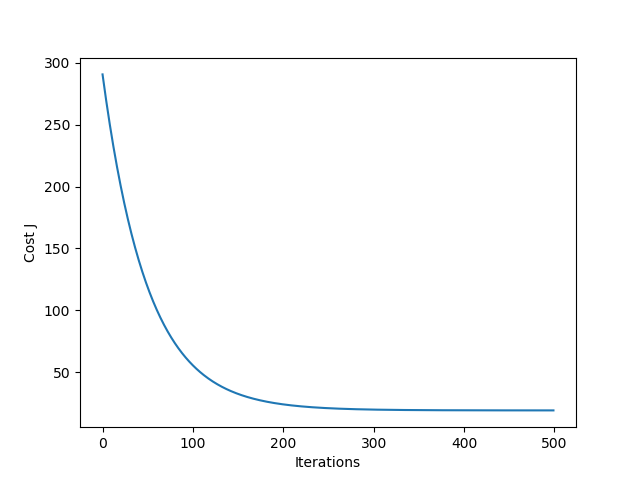
\includegraphics[scale = 0.5]{cost_function}
 \captionsetup{font=scriptsize}
  \caption{Cost function of the baseline model}
\end{figure}

 Out of all 13 features, the percentage of low socioeconomic status in the population (LSTAT) may be the best predictor for housing price ($R_{2}$= 0.54), and it is negatively correlated with the housing prices. In other words, if there is a higher percentage of low status in the population, the housing price may be lower (Figure 2). 
\begin{figure}[!htbp]
 \centering
 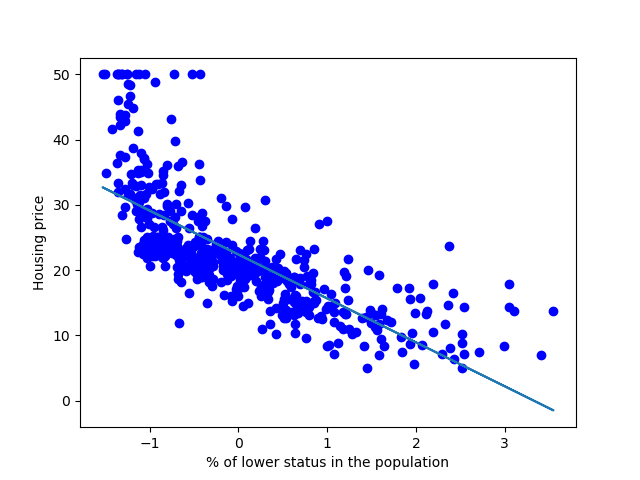
\includegraphics[scale = 0.5]{baseline}
 \captionsetup{font=scriptsize}
  \caption{The baseline model}
\end{figure}


The average number of rooms per dwelling (RM) also correlates highly with the housing price (Figure 3). After adding the feature (RM) to the regression model, we found that $R_{2}$ improved from 0.54 to 0.64.
\begin{figure}[!htbp]
 \centering
 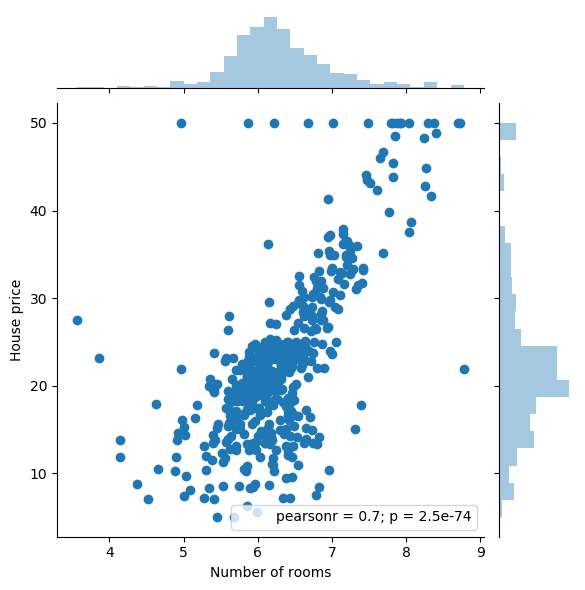
\includegraphics[scale = 0.5]{RM}
 \captionsetup{font=scriptsize}
  \caption[8pt]{Correlation between the average number of rooms per dwelling and housing price}
\end{figure}

Even though some features don't correlate highly with the housing prices, but collectively they can predict the housing price better ($R_{2}$ = 0.73). 

Some features (e.g., DIS, LSTAT) have highly skewed distribution (Figure 4), we did log transformation on those features to make it closer to normal distribution, and that also improved the model fit ($R_{2}$ = 0.79).\\

\begin{figure}[!htbp]
 \centering
 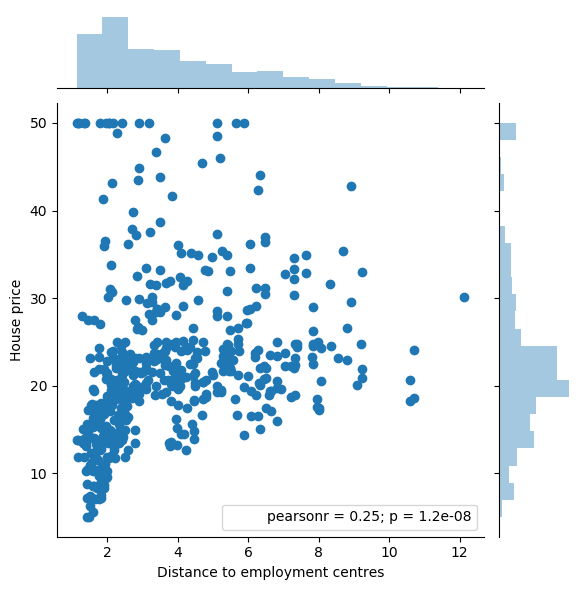
\includegraphics[scale = 0.5]{distance}
 \captionsetup{font=scriptsize}
  \caption[8pt]{Correlation between weighted distances to five Boston employment centres and housing price}
\end{figure}

Table 2 shows the improvements we made to achieve higher $R_{2}$ value.

\begin{table}[!htbp]
\small
\centering
\captionsetup{font=scriptsize}
\caption[8pt]{Evaluation of regression fits ($R^{2}$) for different models}
\begin{tabular}{|c|c|}
 \hline
Model & $R^{2}$ \\
  \hline
LSTAT(Baseline)  & 0.5439\\
LSTAT + RM      & 0.6383 \\
LSTAT + RM + PTRATIO    & 0.6783 \\
All 13 features & 0.7311 \\
log transformation of DIS     & 0.7437 \\
log transformation of DIS, PTRATIO, LSTAT   & 0.7905\\
\hline
\end{tabular}
\end{table}

\section{Conlusion}
In conclusion, some features (e.g., number of rooms, percentage of low status in the population) predicts housing price better than the other features.
As it was expected, not all features accounted for the variance to a very significant extent but we found that the best model we could come up with did include all of the features. 




One significant problem we came across is a frequent one in statistics and machine learning: the bias-variance tradeoff. It is the conflict of simultaneously trying to balance two sources of error, the bias and the variance. While high bias leads to potentially missing relevant relations, high variance can lead to an overly sensitive algorithm and find patterns where there are none. In other words, it is difficult to find the balance between underfitting and overfitting. For future improvement, one could consider using the Bayesian approach to avoid overfitting

The final model accounted for 79 percent of the variance in the data, which is satisfactory, especially considering that some of the features in the dataset did not have a high R2. Cross validation could potentially improve this number, by dividing the training and practicing data better.


\bibliography{eacl2017}
\bibliographystyle{eacl2017}

\end{document}